\documentclass[a4paper]{article}

% Pacotes necessários
\usepackage[portuguese]{babel}
\usepackage[backend=biber, style=apa, citestyle=apa, language=portuguese]{biblatex}
\usepackage{csquotes}
\addbibresource{Recursos/referencias.bib}

\usepackage{amsmath}
\usepackage{graphicx}
\usepackage{subcaption}
\usepackage{setspace}
\usepackage{siunitx}
\sisetup{
  round-mode = places,
  round-precision = 2,
}
\usepackage{enumerate}
\usepackage{enumitem}
\usepackage{karnaugh-map}
\usepackage[section]{placeins}
\usepackage{geometry}
\usepackage{amssymb}
\usepackage{titling}
\usepackage[T1]{fontenc}
\usepackage{float}
\usepackage[hidelinks]{hyperref}
\usepackage{xcolor}
\usepackage{indentfirst}
\usepackage{array}
\usepackage{soul}
\usepackage{afterpage}
\usepackage{makecell}
\newcolumntype{P}[1]{>{\centering\arraybackslash}p{#1}}
\onehalfspacing

% Página de título principal
\newcommand{\firsttitlepage}{
    \begin{titlepage}
        \centering
        \vspace*{1cm}

        \begin{figure}[h!]
            \centering
            
\includegraphics[width=6cm]{Recursos/LOGO_IPB.png}
            \vspace{0.5cm}
        \end{figure}

        \large\textbf{INSTITUTO POLITÉCNICO DE BEJA} \\
        \large\textbf{Escola Superior de Tecnologia e Gestão} \\
        \large\textbf{Mestrado em Engenharia de Segurança Informática} \\
        \large\textbf{Segurança no Software e Usabilidade} \\

        \vspace{2cm}

        {\Huge \textbf{Vaulted Pass™}} \\

        \vspace{1.5cm}

        \large Martinho José Novo Caeiro - 23917 \\
        \large Paulo António Tavares Abade - 23919 \\
        \large Rafael Conceição Narciso - 24473 \\

        \vfill

        \begin{figure}[h!]
            \centering
            
\includegraphics[width=6cm]{Recursos/IPBejaESTIG.jpg}
        \end{figure}

        {\large Beja, junho de 2026}
    \end{titlepage}
}

% Segunda página de título
\newcommand{\secondtitlepage}{
    \begin{titlepage}
        \centering
        \vspace*{1cm}

        \large\textbf{INSTITUTO POLITÉCNICO DE BEJA} \\
        \large\textbf{Escola Superior de Tecnologia e Gestão} \\
        \large\textbf{Mestrado em Engenharia de Segurança Informática} \\
        \large\textbf{Segurança no Software e Usabilidade} \\

        \vspace{2cm}

        {\Huge \textbf{Vaulted Pass™}} \\

        \vspace{1.5cm}

        \large Martinho José Novo Caeiro - 23917 \\
        \large Paulo António Tavares Abade - 23919 \\
        \large Rafael Conceição Narciso - 24473 \\
        \vspace{2cm}

        \large Orientadores: \\
        \large Luís Felipe Nobre Horta Batista Garcia \\
        \large Luís Carlos da Silva Bruno \\

        \vfill

        {\large Beja, junho de 2026}
    \end{titlepage}
}

\begin{document}

\pagenumbering{gobble}
\firsttitlepage
\secondtitlepage

\section*{\LARGE\textbf{\textit{Resumo}}}
Este trabalho analisa o desenho de um sistema de autenticação para dispositivos móveis 
centrado no equilíbrio entre segurança e usabilidade. O foco está na proteção contra 
observação direta do PIN, num contexto em que o utilizador desbloqueia frequentemente 
o telemóvel ou aplicações sensíveis em locais públicos.

A partir dessa necessidade foi desenvolvido o protótipo \textit{Vaulted Pass™}, com quatro 
variações de introdução do PIN: teclado padrão, teclado embaralhado, cadeado padrão e 
cadeado embaralhado. O objetivo é comparar formas de autenticação que reduzam a exposição 
do código sem tornar a tarefa demasiado lenta ou difícil de aprender.

\vspace{1cm}
\textbf{Keywords:} autenticação, PIN, usabilidade, \textit{shoulder surfing}, segurança.
\newpage

\section*{\LARGE\textbf{\textit{Abstract}}}
This work analyzes the design of a mobile authentication system focused on balancing security and usability. 
The emphasis is on protecting PIN entry against direct observation in public or semi-public settings.

The resulting prototype, \textit{Vaulted Pass™}, includes four PIN-entry variations: standard keypad, 
scrambled keypad, standard padlock, and scrambled padlock. The goal is to compare authentication 
approaches that reduce exposure without making the task too slow or hard to learn.

\vspace{1cm}
\textbf{Keywords:} authentication, PIN, usability, shoulder surfing, security.

\renewcommand{\contentsname}{Índice}
\renewcommand{\listfigurename}{Índice de Figuras}

\newpage
\doublespacing
\tableofcontents
\newpage
\listoffigures
\doublespacing

\newpage
\pagenumbering{arabic}

\section{Introdução}\label{introducao}
Este trabalho analisa o desenho de um sistema de autenticação para dispositivos móveis centrado no equilíbrio entre segurança e usabilidade. 
O foco está na proteção contra observação direta do PIN, num contexto em que o utilizador desbloqueia frequentemente o telemóvel ou aplicações 
sensíveis em locais públicos.

A partir dessa necessidade foi desenvolvido o protótipo \textit{Vaulted Pass™}, com quatro variações de introdução do PIN: teclado padrão, 
teclado embaralhado, cadeado padrão e cadeado embaralhado. O objetivo é comparar formas de autenticação que reduzam a exposição do código 
sem tornar a tarefa demasiado lenta ou difícil de aprender.

\section{Revisão Bibliográfica}
Foram analisados três trabalhos científicos diretamente relacionados com autenticação por PIN resistente a observação.

O primeiro artigo, \textit{A PIN-entry method resilient against shoulder surfing}, de Roth, Richter e Freidinger, propõe métodos alternativos 
de entrada de PIN baseados em \textit{cognitive trapdoor games} (\cite{roth2004pin}). A ideia central é dificultar a captura do PIN mesmo 
quando o atacante observa todo o processo de entrada, incluindo gravações em vídeo. Os autores estudam simultaneamente segurança e usabilidade 
e concluem que é possível aumentar de forma relevante a resistência a ataques de \textit{shoulder surfing} sem destruir por completo a 
viabilidade prática do método. Para este projeto, o principal contributo do artigo foi mostrar que a interface pode alterar significativamente 
o nível de exposição do PIN, mesmo mantendo a mesma credencial.

O segundo artigo, \textit{A rotary PIN entry scheme resilient to shoulder-surfing}, apresenta um esquema de entrada do PIN do tipo "roda giratória" 
que também resiste à observação humana e a gravações curtas (\cite{rotary2009}). O trabalho mostra duas variantes da solução e 
procura um compromisso entre segurança e esforço de interação. O resultado mais relevante para este relatório é a demonstração de 
que um mecanismo visual e rotativo pode ser compreendido pelo utilizador após curta aprendizagem, ao mesmo tempo que reduz a utilidade 
de um ataque por observação. Este princípio foi usado no desenho da variante em forma de cadeado do protótipo.

O terceiro artigo, \textit{Visual Attention and Learning Effects in Shoulder-Surfing: A Human-Factors Perspective on PIN Observation} (\cite{visualattention2026}), analisa 
como funciona a atenção visual e o fator de aprendizagem para quem observa a introdução de um PIN, nomeadamente, os espiões de ombro. O artigo 
considera sempre um PIN de 4 dígitos mas altera diversas variáveis como as condições ambientais, as técnicas de ocultação por parte dos utilizadores, 
os efeitos de aprendizagem e ainda as características demográficas dos observadores. Os autores concluíram que o efeito de aprendizagem é o maior perigo, 
e quantas mais vezes se observa a introdução do PIN, mais fácil se torna para o atacante memorizar a sequência. É destacado pelos autores que a atenção é focada 
nos movimentos e não só no ecrã, então tentar ofuscar o ecrã não é suficiente pois os movimentos da mão denunciam a sequência.

\section{Análise do Sistema}
\subsection{As 11 Questões Fundamentais da Análise de Tarefas}
\begin{enumerate}[label=\arabic*.]
    \item \textbf{Quem vai utilizar o sistema?} Utilizadores de smartphones que procuram maior privacidade e segurança, abrangendo 
    desde pessoas tecnologicamente avançadas até utilizadores com reduzida literacia digital ou séniores.
    \item \textbf{Que tarefas executam atualmente?} Desbloqueio de dispositivos e aplicações por métodos biométricos (impressão digital, 
    reconhecimento facial) ou por PIN/senhas, frequentemente em espaços onde terceiros podem observar o ecrã.
    \item \textbf{Que tarefas são desejáveis?} Autenticação robusta que proteja dados sensíveis (bancários, saúde, mensagens) contra 
    observadores externos, mantendo memorização e rapidez no acesso.
    \item \textbf{Como se aprendem as tarefas?} Por experimentação direta e através de um curto tutorial inicial (onboarding) que 
    explica a lógica dos métodos embaralhados e rotativos.
    \item \textbf{Onde são desempenhadas as tarefas?} Em contextos móveis: transportes públicos, cafés, filas, ruas — ambientes com 
    risco de observação lateral.
    \item \textbf{Qual a relação entre o utilizador e a informação?} O utilizador é o titular legítimo dos dados; o sistema atua 
    como gatekeeper, validando a identidade antes de liberar acesso.
    \item \textbf{Que outros instrumentos tem o utilizador?} Ecrã tátil do smartphone, memória visual/motora e, opcionalmente, 
    acessórios (stylus) ou funcionalidades de acessibilidade do SO.
    \item \textbf{Como comunicam os utilizadores entre si?} A autenticação é individual; contudo, o desenho deve prevenir que a 
    observação de entradas revele a senha.
    \item \textbf{Qual a frequência de desempenho das tarefas?} Elevada — o desbloqueio é recorrente ao longo do dia, exigindo 
    soluções eficientes e pouco intrusivas.
    \item \textbf{Quais as restrições de tempo impostas?} A autenticação deve ser rápida (idealmente < 30s). Em caso de várias 
    tentativas falhadas, deve aplicar-se um tempo de espera para mitigar ataques.
    \item \textbf{Que acontece se algo correr mal?} Feedback imediato ao utilizador (ex.: "PIN Incorreto"); em falhas repetidas, 
    mecanismos de recuperação (email, código mestre) e registo de tentativas suspeitas.
\end{enumerate}

\subsection{Caracterização dos Utilizadores}
Os utilizadores-alvo podem ser caracterizados como pessoas com uso frequente de smartphone e aplicações pessoais sensíveis. 
Há três perfis especialmente relevantes: utilizadores jovens e tecnologicamente confortáveis, que valorizam rapidez; utilizadores 
adultos que procuram um equilíbrio entre segurança e conveniência; e utilizadores seniores, que beneficiam de interfaces mais 
explícitas e de menor carga de memória.

Em termos de contexto, o nível de escolaridade e a formação em informática variam bastante, pelo que o sistema não pode depender 
de conhecimento técnico prévio. Se fosse possível contactar utilizadores e organizações, seria importante recolher dados sobre 
frequência de utilização do telemóvel, experiências anteriores com métodos de autenticação, dificuldades de acessibilidade, tempo 
aceitável para desbloqueio e perceção real de risco em espaços públicos.

Caso fosse possível estabelecer um contacto direto e formal com os utilizadores, a recolha de informação detalhada 
seria estruturada através de uma abordagem mista. Em primeiro lugar, seria aplicado um \textit{inquérito por questionário} 
digital (Microsoft Forms), focado em mapear quantitativamente a perceção de risco de \textit{shoulder surfing} considerando a 
opinião dos utilizadores.

Em segundo lugar, para obter dados qualitativos e contextuais profundos, seriam realizadas 
\textit{entrevistas semiestruturadas} com amostras de utilizadores das três faixas etárias 
identificadas, permitindo explorar as suas reais dificuldades de acessibilidade com tecnologia móvel. 
Por fim, planear-se-ia uma \textit{observação direta de campo} (estudo etnográfico discreto) em locais 
de grande afluência da cidade de Beja, como paragens de autocarro e cafés, para registar os comportamentos 
espontâneos de ocultação física do ecrã que os utilizadores adotam no seu quotidiano.

\newpage
\subsection{Cenários de Utilização}

\textbf{Persona 1: Ricardo (O Analista Urbano)}
\begin{itemize}
    \item \textbf{Perfil:} 28 anos, tecnológico, vive em Lisboa e usa transportes públicos.
    \item \textbf{Cenário:} O Ricardo está num metro lotado e precisa de consultar o saldo bancário. Tem receio que alguém ao seu lado memorize o seu PIN.
    \item \textbf{Aplicação no protótipo:} Utiliza o \textit{PIN Baralhado}. Como os números mudam de posição a cada acesso, mesmo 
    que alguém observe o movimento dos dedos, não conseguirá replicar a sequência noutra sessão.
\end{itemize}

\textbf{Persona 2: Dona Maria (A Utilizadora Sénior)}
\begin{itemize}
    \item \textbf{Perfil:} 72 anos, reformada, com dificuldades visuais.
    \item \textbf{Cenário:} Deseja desbloquear o telemóvel para mostrar fotografias a familiares, mas sofre com a leitura de pequenos dígitos.
    \item \textbf{Aplicação no protótipo:} Utiliza o \textit{PIN em Forma de Cadeado}. Ao rodar o número de vezes necessárias a 
    partir do ponto zero, recorre à memória gestual, tornando o acesso mais intuitivo e menos stressante.
\end{itemize}

\textbf{Persona 3: Tiago (O Estudante Dinâmico)}
\begin{itemize}
    \item \textbf{Perfil:} 21 anos, estudante de engenharia, em movimento constante.
    \item \textbf{Cenário:} Corre para a faculdade com mochila e precisa de validar um bilhete digital enquanto caminha entre a multidão.
    \item \textbf{Aplicação no protótipo:} Utiliza o \textit{PIN Forma Cadeado Baralhado}. É a variante de segurança máxima: exige rodar 
    o cadeado enquanto os números estão em posições aleatórias, reduzindo a possibilidade de decifração por observadores distantes.
\end{itemize}

\newpage
\subsection{Análise de Tarefas}
A tarefa principal é autenticar o utilizador com um PIN sem expor o código a observadores.

\textbf{Sequência de Tarefas:}
\begin{enumerate}
    \item \textbf{Pre-Configuração:} \nobreak\par
    \begin{enumerate}
        \item Definir o PIN numérico.
        \item Escolher o tipo de PIN: Normal, Baralhado, Forma Cadeado, ou Forma Cadeado Baralhado.
    \end{enumerate}
    \item \textbf{Processo de Autenticação (rotina diária):} \nobreak\par
    \begin{enumerate}
        \item Ativar o ecrã de desbloqueio (abrir a app ou ligar o ecrã).
        \item Observar a disposição do teclado (identificar se os números estão na posição padrão ou baralhados).
        \item Introduzir os dígitos ou rodar a "forma de cadeado" conforme a lógica do método ativo.
        \item Submeter a tentativa de acesso (automático ao atingir o número de dígitos ou via botão "OK").
    \end{enumerate}
\end{enumerate}

Nos métodos tradicionais a tarefa é direta, mas mais vulnerável a observação; nos métodos embaralhados, o utilizador interpreta a 
disposição atual dos números; na variante em forma de cadeado, a ênfase passa para a memória gestual e no feedback visual dos dials. 
Em caso de erro, o sistema permite corrigir a tentativa e fornece feedback imediato sem penalizar indevidamente o utilizador legítimo.

\newpage
\subsection{Versão Base: Autenticação por PIN com Teclado Digital Estático}
Esta versão representa o método convencional, com teclado fixo e ordenação previsível dos números. É a solução mais rápida e familiar, 
mas também a mais vulnerável a \textit{shoulder surfing}, gravação por câmara e observação lateral. Serve como base de comparação para 
medir o custo de segurança das restantes variantes.

\subsection{Primeira Variante: Autenticação por PIN com Teclado Digital Embaralhado}
A primeira variante altera a posição dos números em cada acesso. O objetivo é reduzir a utilidade da observação visual, porque um atacante 
que memorize a posição dos toques numa sessão terá dificuldade em repetir a sequência noutra sessão. Esta solução mantém a lógica clássica 
do PIN, mas obriga o utilizador a olhar para o teclado em cada autenticação.

\subsection{Segunda Variante: Autenticação por PIN com Forma de Cadeado Estática}
A variante em forma de cadeado traduz a introdução do PIN para um mecanismo visual de rotação. Em vez de tocar diretamente em botões fixos, 
o utilizador ajusta cada dígito até ao valor pretendido. A vantagem é tornar a leitura do código menos óbvia para um observador, ao mesmo 
tempo que introduz uma associação visual mais forte entre ação e número.

\subsection{Terceira Variante: Autenticação por PIN com Forma de Cadeado Embaralhada}
Na variante embaralhada da forma de cadeado, a disposição dos números muda, aumentando ainda mais a resistência à observação. Em contrapartida, 
o esforço cognitivo cresce, pelo que o desenho deve privilegiar feedback claro, legibilidade e consistência.

\section{Desenho do Sistema}
\subsection{Interfaces dos Equipamentos Físicos e Ecrãs}
O protótipo foi desenhado para simular uma aplicação móvel simples, com três ecrãs principais: configuração inicial, ecrã de autenticação e 
ecrã de resultado.

No ecrã inicial o utilizador escolhe o PIN e a variante de autenticação. No ecrã de teste é apresentada a interface correspondente à variante 
selecionada, com teclado numérico ou dials em forma de cadeado. No ecrã final surge o tempo de execução, a variante usada e o resultado da tentativa.

As interfaces físicas foram pensadas para comunicação clara e baixo ruído visual, com foco nos elementos essenciais: identificação do método, 
introdução do PIN, botão de confirmação e feedback de erro ou sucesso.

\begin{figure}[H]
    \centering
    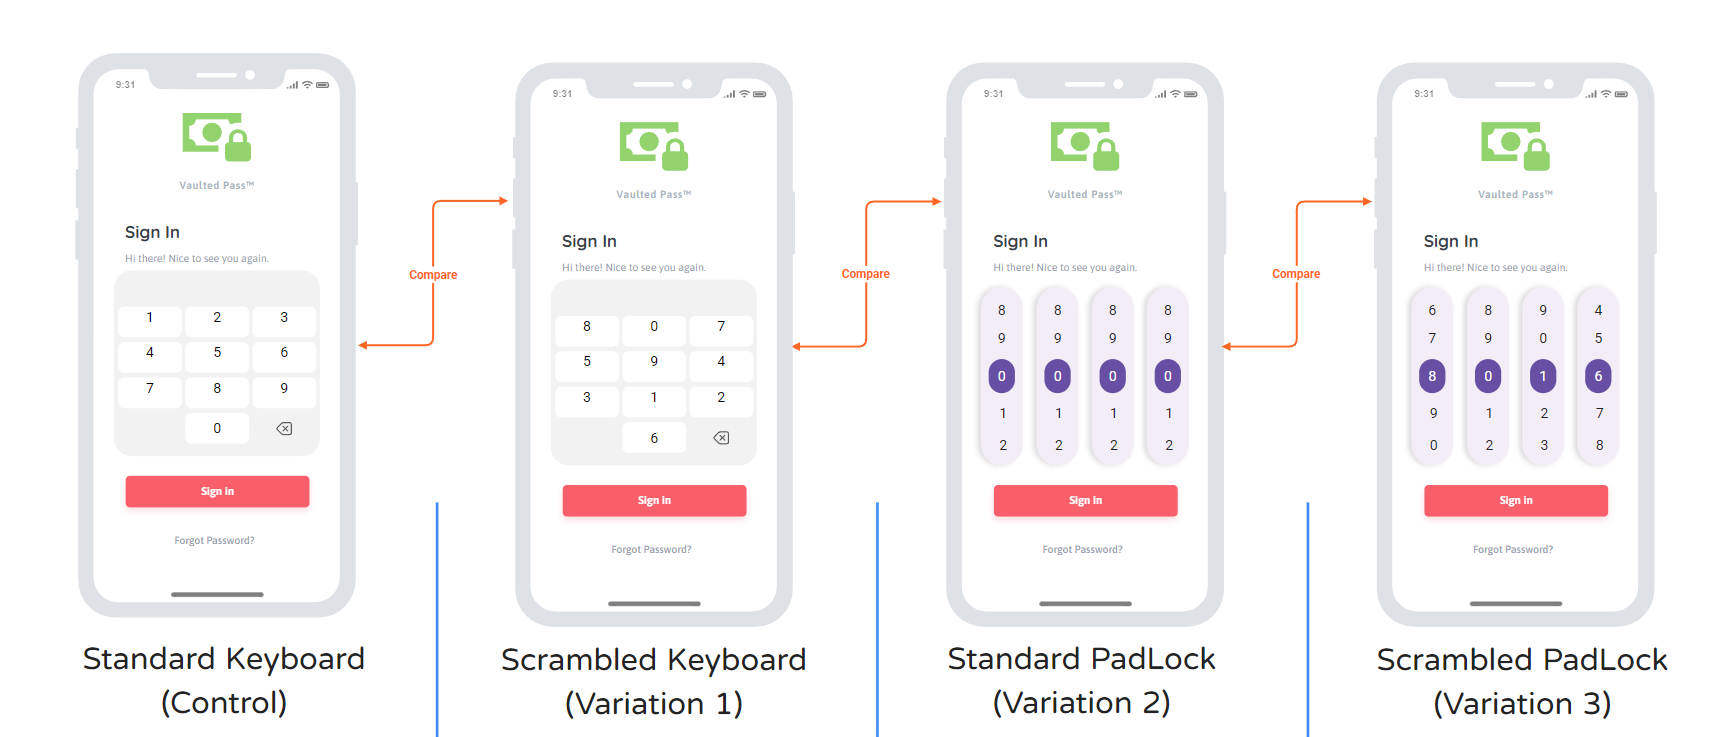
\includegraphics[width=0.95\linewidth]{../Wireframes/Medium Fidelity.png}
    \caption{Protótipo de média fidelidade da aplicação.}
\end{figure}

\newpage
\subsection{Diagramas de Navegação}
O fluxo principal do sistema é linear: configuração inicial $\rightarrow$ autenticação $\rightarrow$ resultado $\rightarrow$ regresso ao menu inicial. 
Em caso de erro no PIN, o utilizador permanece no ecrã de autenticação e pode corrigir a introdução antes de confirmar novamente.

Esta navegação simples reduz a carga de aprendizagem e evita que o utilizador tenha de memorizar caminhos complexos entre ecrãs. Como o objetivo do 
projeto é avaliar o método de entrada do PIN e não a exploração da aplicação, a estrutura de navegação foi mantida intencionalmente curta.
\begin{figure}[H]
    \centering
    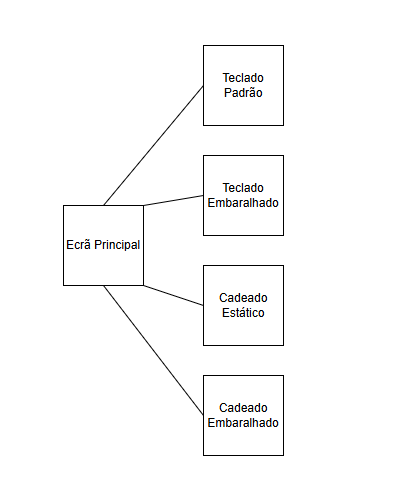
\includegraphics[width=0.40\linewidth]{Recursos/diagramanavegacao.png}
    \caption{Diagrama de navegação do protótipo.}
\end{figure}
\subsection{Princípios e Regras de Usabilidade}
Foram aplicados vários princípios de usabilidade considerados centrais neste projeto:
\begin{itemize}
    \item \textbf{Visibilidade do estado do sistema:} o temporizador e o ecrã de resultado mostram sempre o estado atual da interação.
    \item \textbf{Consistência:} os botões, cores e linguagem visual mantêm-se entre as variantes.
    \item \textbf{Prevenção de erros:} o campo do PIN aceita apenas dígitos e o sistema pede confirmação explícita.
    \item \textbf{Reconhecimento em vez de memória:} os métodos visuais mostram o valor atual de forma direta, reduzindo a necessidade de recordar 
    passos anteriores.
    \item \textbf{Feedback imediato:} cada tentativa termina com indicação clara de sucesso ou falha.
    \item \textbf{Simplicidade:} a interface evita opções desnecessárias e concentra-se na tarefa principal.
\end{itemize}

Além destes princípios, o desenho procurou respeitar a legibilidade e a robustez da interação em ecrãs pequenos, privilegiando controlos grandes 
e um contraste visual suficiente para uso em contexto móvel.

\subsection{Avaliação Exploratória do Protótipo Não Funcional}
Foi pedido a três possíveis utilizadores que interagissem com o protótipo 
de média fidelidade, sem instruções detalhadas, para observar a sua capacidade de 
compreender a lógica. Foi apenas pedido para que escolhessem aquela 
variante que considerassem a mais segura e mais eficiente. A variante mais votada 
foi a de teclado embaralhado, seguida da variante em forma de cadeado.

\begin{figure}[H]
    \centering
    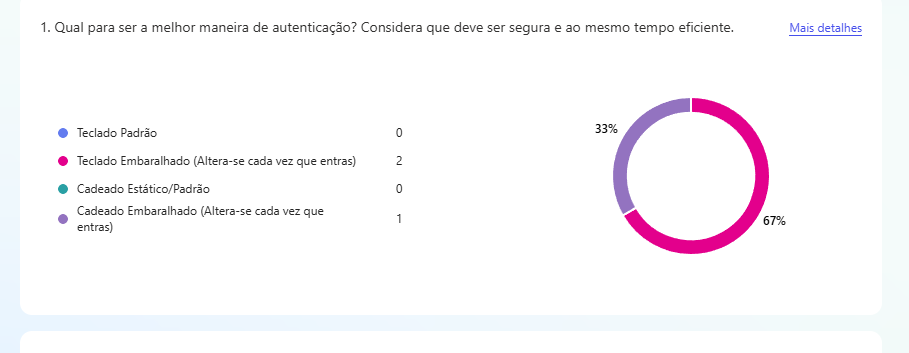
\includegraphics[width=0.60\linewidth]{Recursos/naofuncional.png}
    \caption{Avaliação do protótipo não funcional.}
\end{figure}

Os utilizadores mencionam que ao manter a familiaridade com o teclado padrão, mas aumentando 
a segurança com o embaralhamento, impedindo que mesmo que se vejam os movimentos da mão, 
não se consegue replicar a sequência noutra sessão. A variante em forma de cadeado foi 
considerada interessante também, por ser mais confusa para um observador e fará com isso 
seja mais difícil de memorizar a sequência.

\newpage
\section{Implementação e Avaliação do Protótipo}
\subsection{Implementação do Protótipo}
O protótipo funcional foi implementado em Python com Kivy, usando \texttt{ScreenManager} para alternar entre o ecrã de configuração, o ecrã de 
teste e o ecrã de resultado. A lógica principal separa quatro modos: teclado padrão, teclado embaralhado, cadeado padrão e cadeado embaralhado.

O teclado numérico é gerado dinamicamente e, na variante embaralhada, a ordem dos números é aleatorizada em cada sessão. Na variante em forma 
de cadeado, o utilizador interage com dials verticais, o que permite simular uma entrada mais visual e menos dependente da leitura direta do teclado.

O protótipo mede o tempo de execução, regista o melhor desempenho por modo e apresenta feedback imediato após cada tentativa. Estas decisões 
foram tomadas para suportar uma avaliação comparativa da interface e do comportamento do utilizador.

\subsection{Avaliação do Protótipo}
O protótipo já permite avaliar diferenças de desempenho entre os vários modos, tanto em termos de rapidez como de facilidade de compreensão. A 
versão padrão serve como referência de comparação, enquanto as variantes embaralhada e em cadeado permitem estudar o impacto de mecanismos de 
segurança adicionais na interação.

Para uma avaliação final com utilizadores, deverá ser recolhido o tempo de execução, o número de erros, a preferência subjetiva e a perceção de 
segurança. Esses dados permitirão discutir se o aumento de proteção justifica o esforço adicional imposto pela interface.

\newpage
\section{Testes com Utilizadores}
Foram realizados testes com um grupo de 6 utilizadores, com idades entre 22 e 57 anos, todos com alguma experiência em smartphones. Para 
cada participante foi explicado previamente o objetivo do teste e foi fornecido o guião de tarefas. 
Cada utilizador experimentou as quatro variantes do protótipo, e foram registados o tempo de execução, o número de erros e a preferência subjetiva.


\begin{table}[H]
\centering
\setlength{\tabcolsep}{4pt} % Ajuste fino para caber na página
\small
\begin{tabular}{|c|c|c|c|c|c|c|c|c|}
\hline
\textbf{Utilizador} & 
\textbf{\makecell{Tempo\\TP (s)}} & 
\textbf{\makecell{Erros\\TP}} & 
\textbf{\makecell{Tempo\\TEmb (s)}} & 
\textbf{\makecell{Erros\\TEmb}} & 
\textbf{\makecell{Tempo\\CEst (s)}} & 
\textbf{\makecell{Erros\\CEst}} & 
\textbf{\makecell{Tempo\\CEmb (s)}} & 
\textbf{\makecell{Erros\\CEmb}} \\
\hline
Utilizador J & 4.23 & 0 & 3.55 & 0 & 7.63 & 2 & 9.61 & 0 \\
Utilizador H & 3.22 & 0 & 4.47 & 0 & 5.96 & 2 & 6.49 & 1 \\
Utilizador M & 3.42 & 0 & 5.31 & 0 & 7.61 & 0 & 5.79 & 0 \\
Utilizador S & 1.26 & 0 & 2.28 & 0  & 8.51 & 0 & 9.20 & 0 \\
Utilizador T & 2.58 & 0 & 2.45 & 0 & 4.20 & 0 & 7.34 & 1 \\
Utilizador P & 3.64 & 0 & 6.19 & 0 & 42.22 & 9 & 32.53 & 36 \\
\hline
\hline
\textbf{Média} & 2.89 & 0.00 & 4.04 & 0.00 & 12.69 & 2.17 & 11.83 & 6.33 \\
\textbf{Mediana} & 3.32 & 0.00 & 4.01 & 0.00 & 7.62 & 1.00 & 8.27 & 0.50 \\
\textbf{Desvio Padrão ($\sigma$)} & 1.07 & 0.00 & 1.54 & 0.00 & 14.53 & 3.43 & 10.25 & 14.54 \\
\hline
\end{tabular}
\caption{Resultados expandidos dos testes com utilizadores ($N=6$).}
\label{tab:resultados_testes}
\end{table}

A análise dos dados estatísticos descritivos da Tabela~\ref{tab:resultados_testes} revela um fenómeno 
crítico no domínio da Interação Pessoa-Computador: o impacto de \textit{outliers} em amostras pequenas ($N=6$).

O \textbf{Teclado Padrão (TP)} apresentou a menor média de tempo ($2.89$\,s) e elevada consistência ($\sigma = 1.07$\,s), 
justificável pela familiaridade universal com o método. O \textbf{Teclado Embaralhado (TEmb)} demonstrou um acréscimo 
marginal no tempo médio ($4.04$\,s) com desvio padrão reduzido ($\sigma = 1.54$\,s) e taxa nula de erros, validando-se 
como uma alternativa altamente usável e previsível.

O cenário altera-se drasticamente nas variantes de cadeado. A média de tempo do \textbf{Cadeado Estático (CEst)} 
disparou para $12.69$\,s com um desvio padrão massivo de $14.53$\,s. Esta distorção é provocada inteiramente 
pelo desempenho do \textbf{Utilizador P}, que registou $42.22$\,s e 9 erros em CEst, escalando para $32.53$\,s 
e $36$ erros no \textbf{Cadeado Embaralhado (CEmb)}. 

Ao analisarmos a \textbf{Mediana}, que mitiga o efeito destes valores extremos, percebe-se que o 
desempenho típico do utilizador no Cadeado Estático ($7.62$\,s) e Cadeado Embaralhado ($8.27$\,s) é 
substancialmente mais baixo do que a média aritmética sugere. O colapso na usabilidade sofrido pelo Utilizador 
P (perfil sénior, com menor literacia digital) evidencia que os mecanismos rotativos geram uma carga 
cognitiva excessiva para determinados nichos de utilizadores, gerando ciclos repetitivos de erro-correção.



Os utilizadores demonstraram uma preferência clara sobre o teclado embaralhado, e o maior consenso foi 
que a variante em forma de cadeado, embora interessante como solução, exigia mais tempo e esse tempo extra podia 
ser um fator que poderia facilitar a observação do PIN e posteriormente a sua memorização. Os utilizadores 
mencionam que apesar de a variante de teclado embaralhado não permitir movimentos memorizados, 
o seu tempo de execução é mais rápido e dificulta a observação do PIN.  Alguns utilizadores ainda mencionaram 
que por questão de conveniência, preferem ainda o teclado padrão, mas que a variante de teclado embaralhado é a 
que oferece maior segurança e que deveria ser incentivada para utilização. As variantes em forma de cadeado, apesar 
de interessantes devido à pouca familiaridade com o método, foram consideradas mais ineficientes e menos agradáveis 
de utilizar. 
\begin{figure}[H]
    \centering
    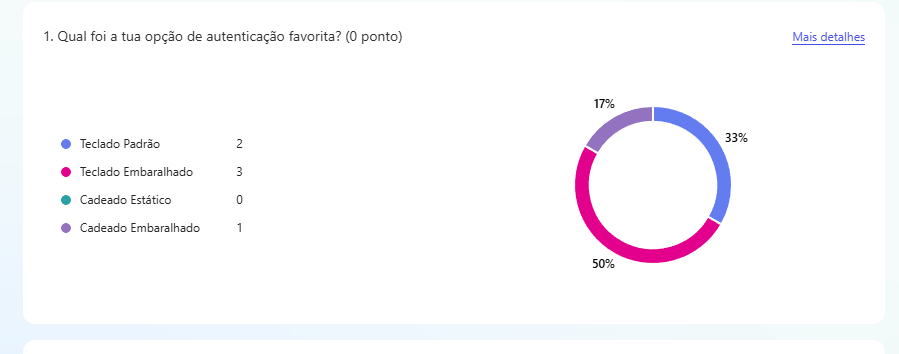
\includegraphics[width=0.95\linewidth]{Recursos/Resultados.png}
    \caption{Resultados dos testes com utilizadores.}
\end{figure}

Por fim, após a análise dos resultados, conclui-se que a variante de teclado embaralhado, é aquela que 
oferece o melhor equilíbrio entre segurança e usabilidade, sendo a mais recomendada para utilização em 
contextos onde a proteção do PIN é uma prioridade. 
\newpage
Originalmente, foi considerada a seguinte ordem 
em termos de segurança: \textit{Cadeado Embaralhado}> \textit{Teclado Embaralhado}  > \textit{Cadeado Estático} 
> \textit{Teclado Padrão}. Isto deve-se ao facto de considerar inicialmente que quanto mais a familiaridade 
dos observadores com o método, mais fácil seria para eles memorizarem o PIN. No entanto, os resultados obtidos 
através de conversas com os utilizadores e os próprios utilizadores a testar, demonstram que a variante de teclado embaralhado é a que oferece maior segurança,
seguida do cadeado embaralhado, depois o cadeado estático e por último o teclado padrão. Isto deve-se ao facto de a 
variante de teclado embaralhado, é um pouco mais familiar para os utilizadores, mas faz com que os observadores não consigam 
memorizar o PIN devido à constante mudança da posição dos números, enquanto que a variante de cadeado embaralhado, 
apesar de seguir a mesma lógica, é menos familiar para os utilizadores, o que faz com que o tempo de execução seja 
maior e consequentemente aumenta a possibilidade de observação do PIN e a sua memorização. 

Os resultados e os testes de utilizador podem ser vistos no na pasta \textit{Anexos}, onde se 
encontra o ficheiro \textit{Pós-Teste da Vaulted Pass.xlsx}, com a pasta \textit{Vídeos} com os vídeos de 
cada utilizador a realizar os testes, e por fim o ficheiro onde cada utilizador informa o seu consentimento.

\newpage
\section{Conclusão}\label{conclusao}
O trabalho consolidou uma abordagem de autenticação por PIN centrada na resistência à observação e na comparação entre diferentes estilos 
de interação. A revisão bibliográfica mostrou que existem soluções eficazes para reduzir o risco de \textit{shoulder surfing} sem sacrificar 
totalmente a usabilidade, e o protótipo desenvolvido materializa esses princípios em quatro variantes distintas.


Do ponto de vista do desenho, a principal conclusão é que segurança e usabilidade não são objetivos incompatíveis, 
mas exigem compromissos visíveis na interface. Através da avaliação estatística e qualitativa realizada com os 
utilizadores, confirmou-se que a variante de teclado embaralhado oferece o melhor equilíbrio prático, 
mitigando o risco de \textit{shoulder surfing} sem penalizar severamente a eficiência e a carga cognitiva do utilizador comum.

\nocite{roth2004pin,rotary2009}
\newpage
\vspace{2cm}
\renewcommand{\refname}{Bibliografia}
\renewcommand{\bibname}{Bibliografia}
\addcontentsline{toc}{section}{Bibliografia}
\printbibliography

\end{document}
